\chapter{数据统计}
有的人说统计学并不是真正的数学,因为它总是模棱两可。可是这种模棱两可往往又可以提供确定性的结论,真是矛盾又美丽的东西啊。 \makebox{}\hfill——沃兹基硕德

\section*{学习目标}
\begin{todolist}
 \item 选择特定的数据呈现方式,讨论每种方法呈现数据的优点与不足
 \item 阅读并绘制\gls{stem-leaf}以及两组数据的茎叶图
 \item 阅读并绘制\gls{boxwhisker}
 \item 阅读并绘制\gls{frequencytable}
 \item 阅读并绘制\gls{histogram}
 \item 阅读并绘制\gls{cumulative}
 \item 理解并求算用于描述中心趋势Central Tendency的三种统计值:mean,median,mode
 \item 理解并求算用于描述数据波动Variation的统计值:range,interquartile range,standard deviation
 \item 从数据本身,或者给定的求和$\sum x$,以及$\sum x^2$求算平均数和标准差;
 \item 理解数据coding对平均值和标准差的影响,能够通过coded data和original data的平均值和标准差互相求算
\end{todolist}
\clearpage


\section{呈现数据的方式}
记录数据只是统计学的第一步,接下来还需要对数据进行分析。在分析的过程当中,好的数据呈现方式能够让人更加快速直观地理解隐藏在数据背后的结论,优美的数据可视化info graphics能够保持信息的传递并且依旧可以呈现原始数据。
\begin{figure}[H]
\centering
\includegraphics[width=0.6\textwidth]{world-of-languages-large}
\end{figure}

\subsection*{茎叶图}
虽然茎叶图的名称当中带有一个图字,但是其本质上还是数据,只不过是按照特定的书写格式和排序方式给出所有的原始数据。
如下图所示:
\begin{figure}[H]
\centering
\includegraphics[width=0.4\textwidth]{stemleaf}
\label{fig:stem-and-leaf}
\caption{统计了一个班上身高的茎叶图}
\end{figure}

从茎叶图上可以获得原始数据,并不会发生\textbf{信息损失}:
\begin{table}[H]
\centering
\begin{tblr}{|l|l|l|l|l|l|l|l|l|l|}
\hline
157 & 159 & 160 & 160 & 164 &     &     & 165 & 168 &     \\ \hline
    &     & 169 &     &     & 170 & 173 &     &     & 174 \\ \hline
175 &     &     &     &     & 178 &     & 179 &     & 183 \\ \hline
184 &     &     &     &     &     &     & 196 &     &    \hline
\end{tblr}
\end{table}

\begin{TaskBox}
尝试根据茎叶图,将原始数据统计表填完
\end{TaskBox}

\subsection*{背对茎叶图}
如果将一个班按照性别区分,分别统计每个学生的身高,男生和女生的``茎''都可以是15,16,17,18,19等。因此可以使用back to back stem and leaf diagram,把两组的数据整合到一起。
\begin{figure}[H]
\centering
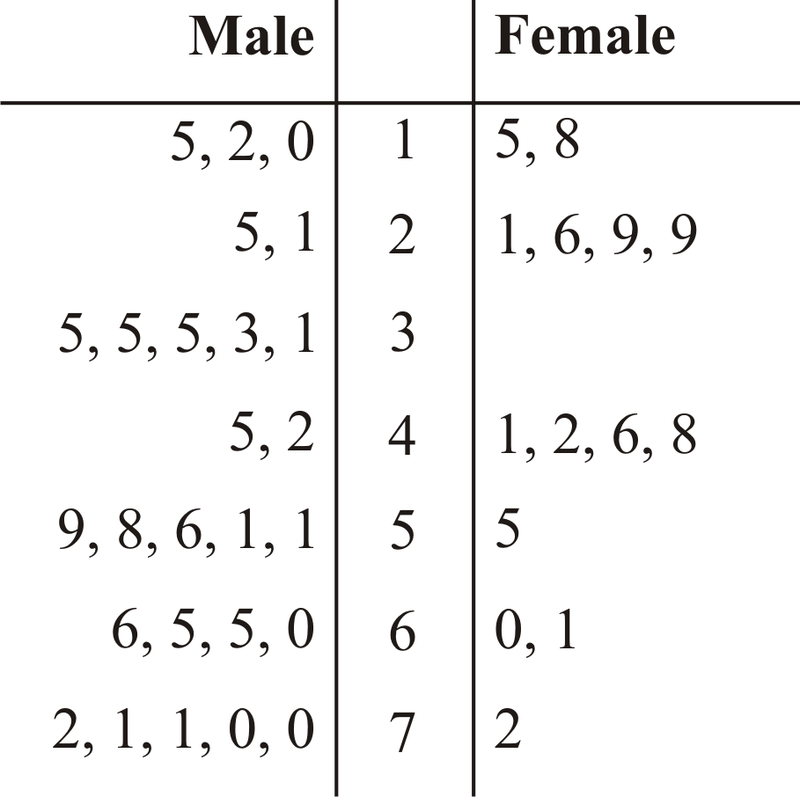
\includegraphics[width=0.4\textwidth]{backtoback}
\caption{背对茎叶图}
\end{figure}
\clearpage


\subsection*{盒须图}
\label{subsec:boxwhiskerplot}
在绘制盒须图之前,需要能够计算如下的五个数据值,最小值,\gls{lower quartile},中位数,\gls{upper quartile},最大值。
计算中位数的\textbf{位置序号}的公式为:
\[
	\frac{n+1}{2}
\]
比如从\ref{fig:stem-and-leaf}当中,有$39$个统计数据,因此中位数的序号就是$(39+1)/2=20$。也就是要找第$20$个数据,没毛病。

但是如果统计的总个数为\textcolor{r1}{偶数}的时候,再次利用公式求算定位会发现,中位数的序号在第$20.5$。遇到这种情况不要慌,只需要选择第$20$个和第$21$个数据值,计算一下两者的平均数就好了。

\subsubsection*{上下四分位数}
四分位数的概念和中位数是近似的,都是代表排序之后的位于特定位置的数据。顾名思义,上四分位数就是比$75\%$的数据更大的那个数据,下四分位数就是比$25\%$的数据更大的那个数据。数学符号上也可以计作$Q_3$和$Q_1$。

\subsubsection*{四分位距}
\gls{IQR}的求算非常简单,其公式就是:
\[
	IQR = Q_3-Q_1
\]
代表着中间一半的数据的波动范围。在\gls{onevariable}IQR也可以被用来来判断是否有\gls{outlier}的存在。
\clearpage


\subsection*{频率分布表}
\subsubsection*{离散频率分布表}
当数据有大量重复的时候,可以将该数据值和数据的次数放在一个表格当中,这样的表格就叫做频率(数)分布表。该表格对信息没有做任何的删减,是可以\textbf{恢复到原始统计数据的}。如下图所示
\begin{figure}[H]
\centering
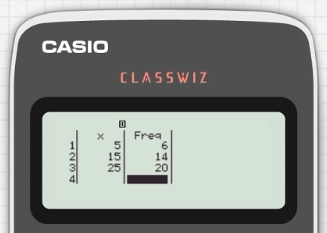
\includegraphics[width=0.5\textwidth]{casio_freq}
\label{fig:casiofreq}
\caption{fx991当中的频率分布表}
\end{figure}
从这张表格当中,我们可以知道原始统计值为5,5,5,5,5,5,15,15,15,15,15,15,15,15,15,15,15,15,15,15,25,25,25,25,25,25,25,25,25,25,25,25,25,25,25,25,25,25,25,25。所以,采用频率表的好处是节省了大量的排序和数数字的工作\footnote{在python的pandas或者collection包当中自带count函数,直接做好类似的工作}。

\subsubsection*{区间频率分布表}
\label{subsubsec:freq distribution}
但是有的时候数据并没有那么完美地重复,比如一个班级的考试成绩,其实61分和62分并没有什么区别,都是处于刚刚飘过的\textbf{区间内}。同理91分和92分也没有区别,因为最后记录GPA的时候都是完美的$4.0$的满绩点。所以,在收集到原始数据之后,可以按照指定的区间进行划分,再将位于特定区间内的数据的总\textbf{频数}累加起来。形成和上面离散型频率分布表类似的表格。但是这种表格就会产生\textbf{数据压缩}。因为是没有办法根据这个表格得到一开始的原始数据的。
\begin{TaskBox}
一个班级40个学生的排序之后的全部成绩为23, 26, 27, 28, 29, 34, 34, 37, 40, 42, 44, 45, 46, 51, 54, 55, 55, 55, 56, 58, 61, 63, 65, 67, 71, 73, 77, 78, 81, 82, 85, 87, 87, 88, 89, 90, 93, 95, 98, 98
尝试以10分为一个区间,补充完下表
\begin{table}[H]
\centering
\begin{tabular}{|c|c|}
\hline
$x$                 & Frequency $f$ \\ \hline
$20\leqslant x< 30$ & 5             \\ \hline
                    &             \\ \hline
                    &             \\ \hline
                    &               \\ \hline
                    &               \\ \hline
                    &               \\ \hline
                    &               \\ \hline
                    &               \\ \hline
\end{tabular}
\end{table}
\end{TaskBox}
因此区间频率分布表本质上也是在做排序和数数的工作。其中每个区间的\gls{classwidth}可以相同(在上题当中都是$10$),也可以不相同。比如低于$60$分的都是不合格,可以将第一个区间写作$20\leqslant x< 60$。这样组距就是$40$了。当然,这一行的频数也会发生对应的增加。

\subsubsection*{累积频率分布表}
这张表格和区间频率分布密切相关,甚至表格形式都几乎一毛一样。但是数据值的含义略有不同。比如还是练习题当中的统计数据,做成累积频率分布表的时候,结果如下
\begin{table}[H]
\centering
\begin{tabular}{|c|c|}
\hline
$x$                 & Cumulative Frequency $\sum f$ \\ \hline
$x< 30$ & 5             \\ \hline
$x< 40$ & 8              \\ \hline
$x< 50$ & 13             \\ \hline
$x< 60$ & 20              \\ \hline
$x< 70$ & 24            \\ \hline
$x< 80$ & 28              \\ \hline
$x< 90$ & 35             \\ \hline
$x< 100$ & 40              \\ \hline
\end{tabular}
\end{table}

不难发现,累积的意思是,只要是小于指定数据的,都需要算进去,因此小于$40$的成绩有$8$个,其中必定包含了小于$30$的那$5$个数据。

\begin{TaskBox}
如何通过\textbf{累积频率分布表}反推区间频率分布表?
\end{TaskBox}
\clearpage

\subsection*{频率分布直方图}
俗话说的好,字不如表,表不如图。尽管表格当中尽可能包含了原始信息。但是不如图像来的那么直观。
因此可以将频率分布表转变为\gls{histogram}。

\subsubsection*{频率密度}
\gls{freqdensity}的定义是单位区间组距上的频率,因此只需要用区间的频率处于组距即可。

\subsubsection*{着手绘制吧}
横坐标的左右端点就是区间的左右端点,纵坐标选择该区间对应的频率密度。绘制一个条形统计图。如下图所示,就是该班的频率分布直方图。
\begin{figure}[H]
\centering
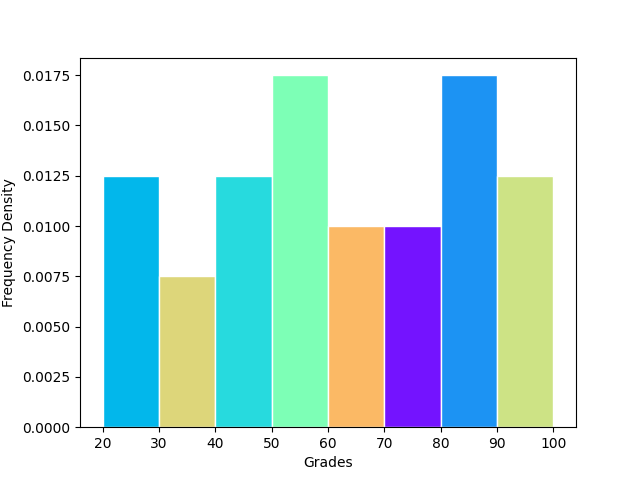
\includegraphics[width=0.8\textwidth]{histogram-matplotlib}
\label{fig:histogram-matplot}
\caption{成绩直方图}
\end{figure}

\begin{SummBox}
频率分布直方图当中,要看清楚纵坐标代表意义到底是频数,还是频率密度。如果是频率密度的话,一定要用\textbf{bar的面积}来计算频数。也就是对应的组距乘以频率密度。
\end{SummBox}
\clearpage

\subsection*{累积频率图}
\gls{cumulative}是根据之前的频率分布表得来的。最终图像为一条曲线。其横坐标依旧为统计变量的取值,纵坐标代表的意义是低于该值的频数,或者百分比。
\begin{TaskBox}
下图为成绩分布累积频率分布图,尝试用光滑曲线连接散点,并利用该曲线,预估整体成绩的中位数
\begin{figure}[H]
\centering
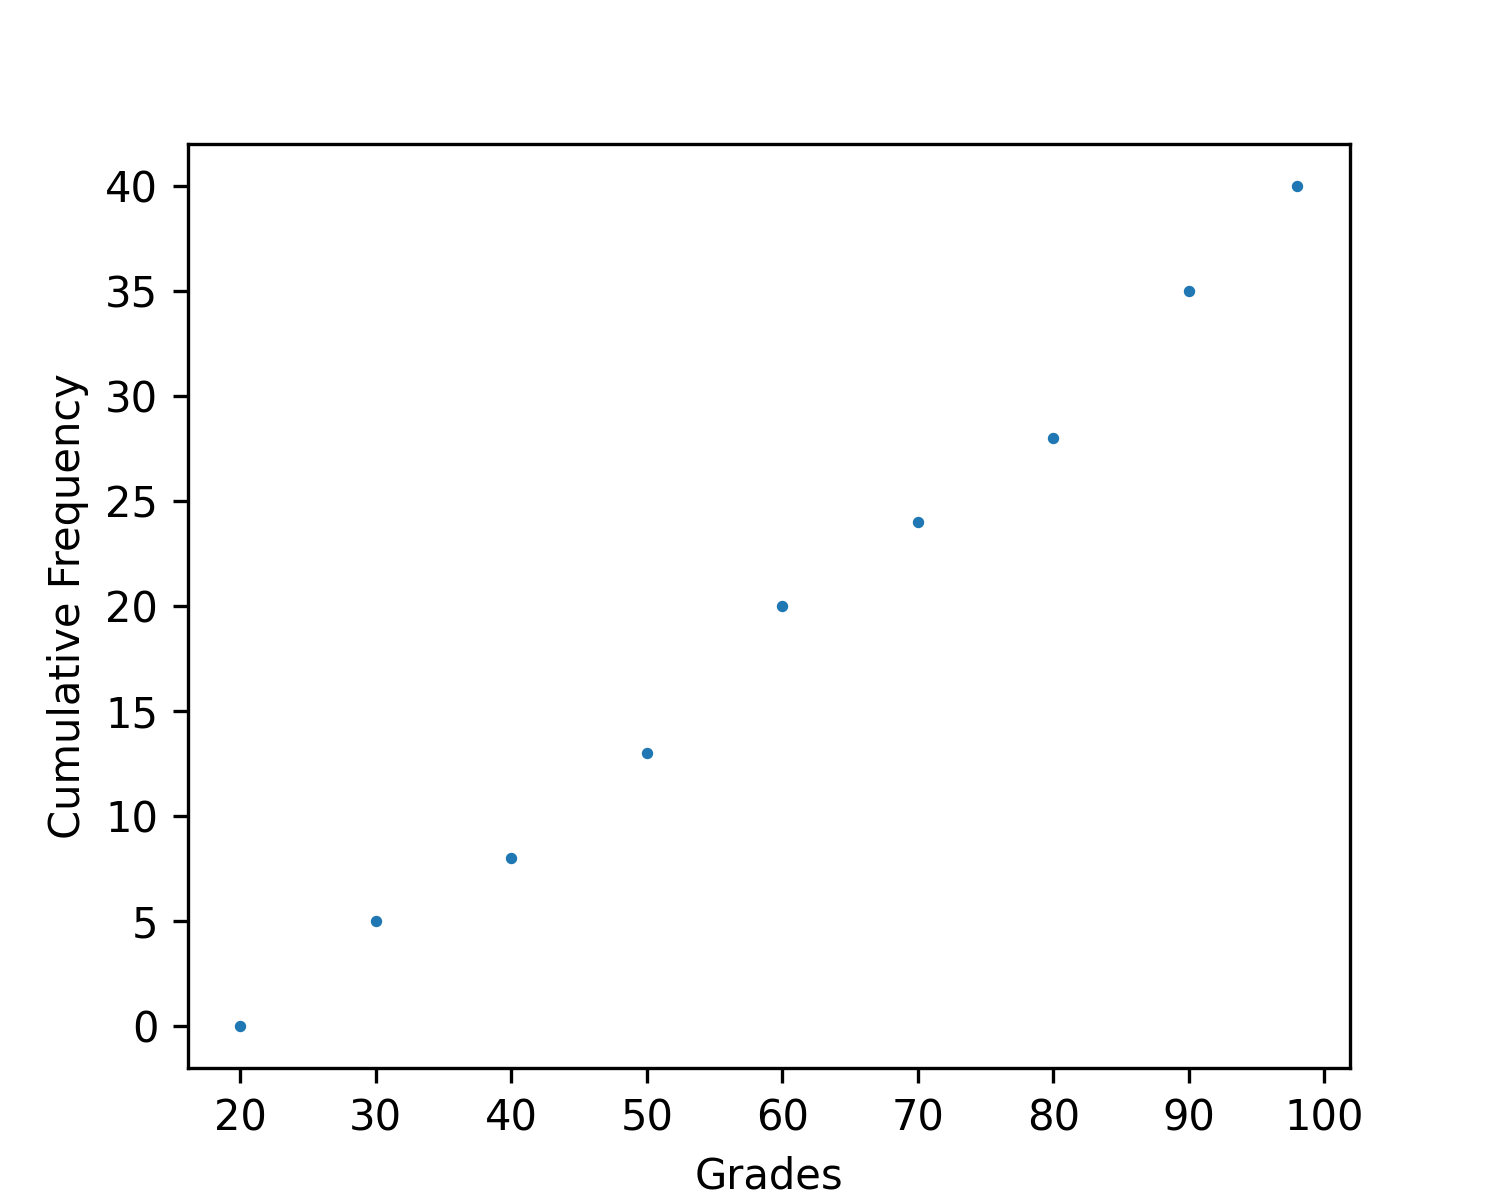
\includegraphics[width=0.8\textwidth]{cumulative}
\end{figure}
\end{TaskBox}
\clearpage

\section{单变量统计计算}
收集数据是第一步,呈现数据是第二步,接下来一个统计学家需要做的事情是用\textbf{定量化}的数字去给出数据最明显的特征。这里的经常考察的特征是两个——数据的\textbf{中心趋势Central Tendency}和\textbf{波动Variation}。

\subsection*{Central Tendency}
常用于衡量一组数据中心趋势的统计值有:\gls{mean},\gls{median},\gls{mode}这三个。

\subsubsection*{中位数}
一组数据排序之后,位于最中间的数据值,和中心趋势当中的中心不谋而合。

\subsubsection*{众数}
一组数据当中\textbf{出现次数最多的数}。因为通常数据是遵循\href{https://open.163.com/newview/movie/free?pid=M82IC6GQU&mid=M83JBLPM4}{中心极限定理},因此众数可以用作描述一组统计数据位于中心的数据。但是这个缺点也是显而易见的:
1.当数据各不相同的时候,不存在众数;
2.数据量比较小的时候,众数可能并不在中间。

\subsubsection*{Modal Class}
对于第一个问题。将数据按照\ref{subsubsec:freq distribution}进行区间划分,可以得到在某些区间内的频数,由此不给出众数的值,而是给出出现次数的数据范围。这样的范围就是modal class。

\subsubsection*{平均数}
在《论语·季氏》当中就提出:不患寡而患不均。这个均字就是平均的意思。也是共产主义社会希望达到的生产资料平均分配的一种体现。那么一组数据的平均数就很好理解了,把全部的统计值相加,再除以总共的数据量。即可得到平均数。其运算公式为:
\[
    \bar{x} = \frac{\sum x}{n}
\]

\subsubsection*{给定频率分布的平均数求算}
对于像\ref{fig:casiofreq}表格当中给定了数据出现频数的统计数据,此时重复的加法就可以变成乘法,因此只需要用每一个数据乘以出现的次数做累加即可。而总的数据个数要把所有的频数相加。公式为:
\[
    \bar{x} = \frac{\sum x\cdot f}{\sum f}
\]

\subsubsection*{区间频率分布的平均数的\textbf{估算}}
如果信息有所省略,用区间频率分布。那么仅需要做一件事,就是用\textbf{区间的中间值}作为重复出现的数据,计算估计的平均值。
\begin{ExampleBox}
1. 一个班级$40$个学生的排序之后的全部成绩为23, 26, 27, 28, 29, 34, 34, 37, 40, 42, 44, 45, 46, 51, 54, 55, 55, 55, 56, 58, 61, 63, 65, 67, 71, 73, 77, 78, 81, 82, 85, 87, 87, 88, 89, 90, 93, 95, 98, 98
求算该班的平均成绩。

2. 如果现在仅提供如\ref{fig:histogram-matplot}频率分布直方图,估计该班的平均成绩
\tcblower
1. 直接套用公式$\bar{x} = \frac{\sum x}{n} = \frac{23+26+\ldots+98+98}{40}=61.6745$

2.首先根据histogram得到对应区间以及频率密度,而后用区间跨度乘以密度得到频率。因此分别为$20\leqslant<30:5$,$30\leqslant<40:3$,$40\leqslant<50:5$,$50\leqslant<60:7$,$60\leqslant<70:4$,$70\leqslant<80:4$,$80\leqslant<90:7$,$90\leqslant<100:5$。第二步,将每个区间的数据全部用中间值替代。利用频率分布的求和公式$\bar{x} = \frac{\sum x\cdot f}{\sum f}=\frac{25\times 5 + 35\times 3+\ldots +95\times 5}{5+3+5+7+4+4+7+5}=61.75$

可以看到,这种方法并不是和真实的平均数一致,但是也非常接近。因此只能叫做\textbf{估算}
\end{ExampleBox}

\begin{TaskBox}
如果区间是间断的,比如计作$20\leqslant x \leqslant 29:5$, $30\leqslant x \leqslant 39:3$的话,需要进行怎样的调整,才能得到一个连续的区间?
\end{TaskBox}

\subsubsection*{对称的分布情况——有用的小结论}
如果绘制histogram,形成类似于下图的情况的话,那么我们可以非常肯定地说,平均数大概在对称轴所处的位置上。
\begin{figure}[H]
\centering
\includegraphics[width=0.5\textwidth]{symmetrical}
\caption{一种比较对称的数据分布}
\end{figure}

\begin{TaskBox}
尝试证明一下图中的结论,即对称式分布的数据,平均数在正中间,和中位数接近(相等)
\end{TaskBox}

\subsection*{Variation}
假设有两只基金,各买入$\$ 10000$,产生的每个月的收益如下:
\begin{table}[H]
\centering
\begin{tabular}{|l|l|l|l|l|l|l|l|l|l|l|l|l|}
\hline
  & Jan & Feb & Mar & Apr  & May  & Jun & Jul  & Aug & Sep & Oct & Nov & Dec \\ \hline
A & $75$  & $-68$ & $15$  & $3$    & $8$    & $97$  & $67$   & $58$  & $32$  & $-35$ & $-42$ & $-64$ \\ \hline
B & $147$   & $776$ & $893$ & $-586$ & $-792$ & $238$ & $-455$ & $21$  & $-72$ & $-87$ & $56$  & $7$ \\ \hline
\end{tabular}
\end{table}
这两只基金在一年的时间内产生的总收益是一样多的。也就是他们的平均月收益都是一样的。但是这两组收益数据具有完全不同的\textbf{波动情况}因此会受到不同种类投资者的选择。A类产品更加适合风险厌恶投资者(Risk Averse Investor),但是B类型的基金就更符合风险偏爱投资者的胃口(Risk Seeking Investor)。所以光给出中心趋势,并不能详尽地给出数据的其他情况,这里的其他情况当中最为重要的就是数据的波动情况。描述一组数据的波动情况可以使用Range, IQR 和 方差与标准差

\subsection*{Range 极差}
这是最简单的描述数据波动的计算值,是用一组数据当中的最大值减去最小值。有一丢丢的作用,但是很明显缺点太多,比如受异常值outlier的影响特别大;不同类型的数据之间比较意义不大, e.g.以\si{cm}为单位统计出的身高,以及以\si{m}作为单位统计出的身高,计算的极差各不相同。但理论上来说是同样的波动的情况。

\subsection*{IQR 四分位距}
为了解决outlier的问题,采用中间$1/2$数据的范围,也就是$Q_3-Q_1$作为用于描述数据波动的计算值,在\ref{subsec:boxwhiskerplot}中已经讨论过,但是这种方法依旧没有摆脱其他数据值的影响。所以也并不会是考试的当中的重点内容。

\subsection*{Variance/Standard Deviation 方差与标准差}
那么有没有什么统计结果可以克服以上的问题,终极的回答是方法与标准差这一对父子\footnote{因为需要先计算方差才能计算标准差,所以说是父子关系}。

\subsubsection*{方差 Var}
\gls{var}的定义公式为:
\[
    \sigma^2_x \text{ or } Var(x)= \frac{\sum(x-\bar{x})^2}{n}
\]
按照公式的理解,就是用统计值减去平均数,得到的就是每个数据和全体中间数据的偏差,然后再将其偏差进行平方化处理(目的是使低于平均数的值带来的负波动非负化),将这些偏差的平方进行累加求和,再除以数据量得到这一组数据的方差。

如果是给定数据频数分布的话,则使用如下的公式:
\[
    \sigma^2_x= \frac{\sum (x-\bar{x})^2\cdot f}{\sum f} 
\]

由于平均数的特殊性质,以上的公式都可以进行展开,化简,得到计算量更小的方差求算公式:
\[
     \sigma^2_x = \frac{\sum x^2}{n} -\bar{x}^2
\]

或者是有频数的时候的公式:
\[
     \sigma^2_x = \frac{\sum (x^2 \cdot f)}{\sum f} -\bar{x}^2
\]

\begin{TaskBox}
1. 尝试证明方差的定义公式展开之后等价于求算公式\\

2. Deep Thinking,如果不进行非负化的处理,直接将正负波动直接相加,最终结果会是多少,为什么?\\

3. 非负化之后的手段除了平方,还有取绝对值,如果用这个定义的话,会有什么优点和什么不足?
\end{TaskBox}


\subsection*{s.d. 标准差}
当求算完方差这个父亲之后,儿子\gls{sd}standard deviation也就出来了。仅需要将求算出的方差,进行开平方根就好了。而标准差在数值上和单位上更接近初始的统计数据,因此会经常被运用于后续的分析

标准差的求算公式:
\[
    \sigma_x= \sqrt {\frac{\sum x^2}{n} -\bar{x}^2}
\]


\subsection*{偏度和峰度}
因此到目前为止,对一个统计数据分布情况,我们可以用平均数来描述中心趋势,用标准差或者方差来描述波动情况,但是这样的精简还不足,后续还有值得讨论但是难度较大的偏度与峰度

\subsubsection*{skewness 偏度}
\gls{skewness}并不是考纲当中的所要求的的点,但是对培养数据的敏感度是非常有用的,不需要掌握求算偏度的\href{https://en.wikipedia.org/wiki/Skewness}{公式},只需要了解,当一组数据的平均数大于其中位数的时候,称这种分布为正偏positively skewed,或者叫做右偏right skewed。反之则成为负偏negatively skewed或者左偏left skewed。

图像如下:
\begin{figure}[H]
\centering
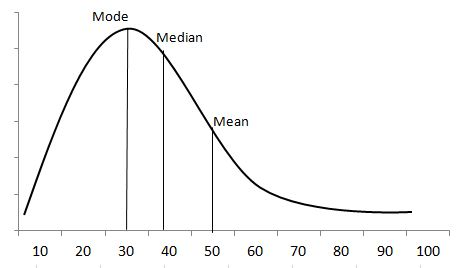
\includegraphics[width=0.4\textwidth]{posskew}
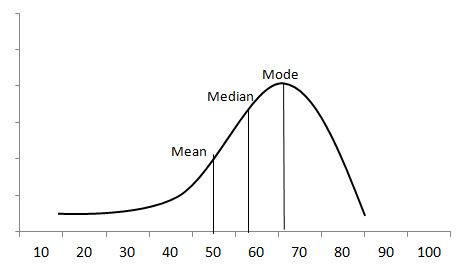
\includegraphics[width=0.4\textwidth]{negskew}
\end{figure}

因此在很多网友调研中,比如上海人均月薪是$¥10,338$这样的统计下,很多微博网友留言表示拖了后腿。其原因在于网友的月收入是positively skewed,收入极高的人频数少,拉高了整体的平均值。如果采用中位数统计的话,该数值会低于平均值。

\subsubsection*{kurtosis 峰度}
\gls{kurtosis}这个概念,可以留作装十三用。当你比别人了解更多的时候,成就感油然而生。同样地也不需要了解\href{https://en.wikipedia.org/wiki/Kurtosis}{公式},该数据值的大小可以用来描述数据分布的集中性程度,也就是中间峰有多高。BTW,\textbf{正态分布}的峰度为$3$。以正态分布的峰度作为基准,可以分为1. Mesokurtic 2. Leptokurtic 3. Platykurtic。感兴趣的可以搜索相关信息
\begin{figure}[H]
\centering
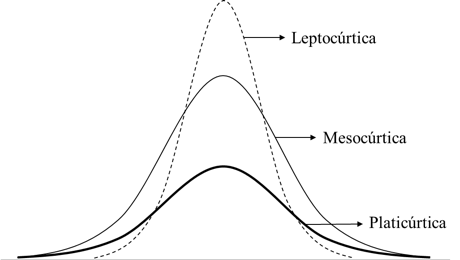
\includegraphics[width=0.9\textwidth]{Kurtosis}
\caption{三种不同峰度的分布图像}
\end{figure}

\begin{figure}[H]
\centering
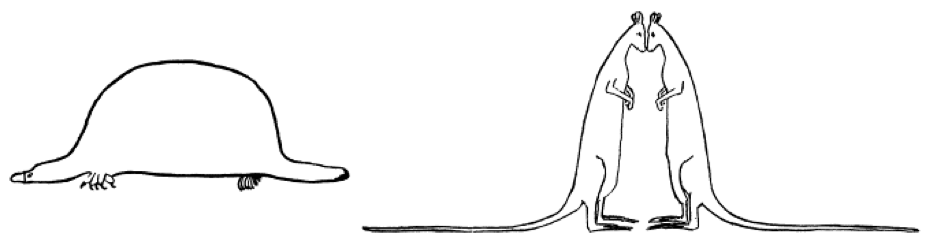
\includegraphics[width=0.8\textwidth]{Kurtosis-interesting}
\caption{一个有趣的模拟图像}
\end{figure}
\clearpage


\section{统计数据值的操作}
先看一条简单的例题:
\begin{ExampleBox}
The ages, $x$ years, of $18$ people attending an evening class are summarized by the following totals:
\[ \sum x = 745  \qquad \sum x^2 =33,951 \]
Find the mean age and standard deviation of the ages in this group of people.

\makebox{}\hfill Adapted from 2004 qp62 Q6 

\tcblower
the mean $\bar{x}=\frac{\sum x}{n}=\frac{745}{18} = 41.38888\ldots \approx 41.4$

the standard deviation $\sigma = \sqrt{\frac{\sum x^2}{n}-\bar{x}^2}=\sqrt{\frac{33951}{18}-41.3888^2} \approx 13.2$
\end{ExampleBox}


好了,这就是在不给定全部数据而是给定数据之和的情况下求算平均数和标准差的基本过程。那么现在对数据进行coding。也就是做了一些调整,产生一组新数据。需要新数据的平均数,方差会和原来的有什么样的关联

\subsection*{数据加减固定值}
比如一个统计为$A$, 另一组统计$B=A+c$。意味着$B$数据组中的所有数据都是由$A$数据组当中的每一个值加c得到的。

\begin{SummBox}
对每个统计值加上或者减去固定数值,新的平均数也是在原来平均数的基础上加上或者减去对应数值,方差没有变动,标准差也没有变动。
\end{SummBox}

\begin{TaskBox}
点击\href{https://www.desmos.com/calculator/sdttllahos}{desmos链接},验证总结的结果

并尝试利用sum notation的方式证明。
\end{TaskBox}


\subsection*{数据值乘以指定倍数}
一组统计为$A$, 另一组统计$C=k\cdot A$。意味着$C$数据组中的所有数据都是由$A$数据组当中的每一个值乘以固定系数$k$得到的。对于这样的数据coding方式,结论是:

\begin{SummBox}
新的平均数也是在原来平均数的基础上乘以$k$,新的方差是原来的方差的$k^2$倍,新的标准差会是原来的$k$倍。
\end{SummBox}

当然,考试不会这么简单,都是具体的含有sum notation的表示方案。

\begin{ExampleBox}
Andy counts the number of emails, $x$, he receives each day and notes that, over a period of $n$ days, $\sum (x − 10) = 27$ and the mean number of emails is $11.5$. and $\sum (x-10)^2 =481$ Find the value of $n$ and the standard deviation of the number of emails.

\makebox{}\hfill Adapted from 2017 winter qp62 Q1
\tcblower
首先,发现coding属于将原有统计值都减去$10$。因此,新的数据的平均数为$11.5-10-1.5$。所以有:
\[
    \frac{\sum (x-10)}{n} =11.5-10 \Longrightarrow \quad n=\frac{27}{1.5}=18
\]

第二个,由于这种coding并不改变标准差的大小,因此新数据的标准差就等同于原有的标准差。所以有:
\[
    \sigma^2 _{x}=\sigma^2 _{x-10} = \frac{\sum{(x-10)^2}}{n}-(\bar{x}-10)^2 = \frac{481}{18}-1.5^2=24.47.
\]
所以标准差就是$\sigma_x=\sqrt{24.47}= 4.95$

因此在没有给定所有数据的情况下,通过coded data也是可以计算原始数据的平均值和方差/标准差等信息的。
甚至,该题还可以反推$\sum x^2$。过程如下:
\[\sum x^2 = (\sigma^2 + \bar{x}^2)\cdot n = (24.47+11.5^2)\times 18 =2821\]
不过需要注意,为得到精确结果,其实带入的时候要尽可能不要选择\textbf{四舍五入的标准差},而是更准确的\textbf{方差}
\end{ExampleBox}
